\documentclass[10pt]{article}
\usepackage[polish]{babel}
\usepackage[utf8]{inputenc}
\usepackage[T1]{fontenc}
\usepackage{amsmath}
\usepackage{amsfonts}
\usepackage{amssymb}
\usepackage[version=4]{mhchem}
\usepackage{stmaryrd}
\usepackage{graphicx}
\usepackage[export]{adjustbox}
\graphicspath{ {./images/} }

\title{LIGA MATEMATYCZNA im. Zdzisława Matuskiego PAŹDZIERNIK 2015 SZKOŁA PODSTAWOWA }

\author{}
\date{}


\begin{document}
\maketitle
\section*{ZADANIE 1.}
Pole trapezu, którego jedna podstawa jest dwa razy dłuższa od drugiej, jest równe \(840 \mathrm{~cm}^{2}\). Oblicz pola trójkątów, na jakie podzieliła ten trapez jedna z przekątnych.

\section*{ZADANIE 2.}
Wykaż, że liczba \(\underbrace{777 \ldots 7}_{90 \text { cyfr } 7}\) jest podzielna przez 45.

\section*{ZADANIE 3.}
Każdy ufoludek ma trzy ręce. Czy 19 ufoludków może się wziąć za ręce tak, aby żadna ręka nie pozostała wolna?

\section*{ZADANIE 4.}
Wszyskie figury składające się na duży prostokąt są kwadratami. Pole czarnego kwadratu jest równe 9. Oblicz długości boków każdego kwadratu i długości boków dużego prostokąta.\\
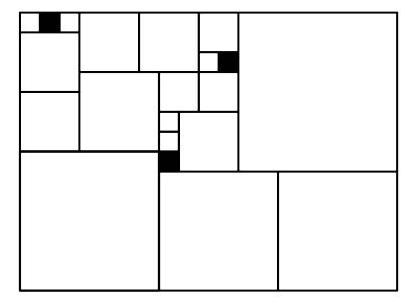
\includegraphics[max width=\textwidth, center]{2024_11_21_868b5a0db8658c5e2e18g-1}

\section*{ZADANIE 5.}
Na terenie wokół jeziora pan Piotr urządził pole namiotowe dzieląc teren na sześć sektorów, jak na rysunku. Pewnej niedzieli przyjechało nad jezioro sześciu wędkarzy, którzy chcieli zamieszkać na polu namiotowym, ale mieli następujące wymagania:

\begin{itemize}
  \item Andrzej nie chce sąsiadować ani z Frankiem, ani z Bartkiem;
  \item Bartek nie chce sąsiadować ani z Andrzejem, ani z Czarkiem;
  \item Czarek nie chce sąsiadować ani z Bartkiem, ani z Damianem;
  \item Damian nie chce sąsiadować ani z Czarkiem, ani z Emilem;
  \item Emil nie chce sąsiadować ani z Damianem, ani z Frankiem;
  \item Franek nie chce sąsiadować ani z Emilem, ani z Andrzejem.
\end{itemize}

Jak rozmieścić wędkarzy, aby spełnić ich życzenia?\\
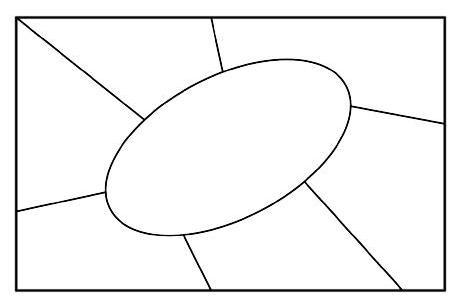
\includegraphics[max width=\textwidth, center]{2024_11_21_868b5a0db8658c5e2e18g-1(1)}


\end{document}